% Generated from the public primitive catalog. Original Atlas drawing; Apache-2.0.
% Target: aes-192; view: overview-compact
\documentclass[border=9pt]{standalone}
% Original Atlas figure theme. Apache-2.0; see the repository LICENSE.
\usepackage[T1]{fontenc}
\usepackage{lmodern}
\usepackage{amsmath,amssymb}
\usepackage{tikz}
\usetikzlibrary{arrows.meta,positioning,calc,fit,backgrounds,decorations.pathreplacing,matrix}
\definecolor{atlasInk}{HTML}{172235}
\definecolor{atlasTeal}{HTML}{0D7B7D}
\definecolor{atlasMuted}{HTML}{637278}
\definecolor{atlasFill}{HTML}{EAF4F2}
\definecolor{atlasLine}{HTML}{B6C8C7}
\tikzset{
  every picture/.style={line width=.65pt,draw=atlasInk,>=Latex},
  every node/.style={text=atlasInk,font=\sffamily\small},
  box/.style={draw,rounded corners=1.5pt,minimum height=.9cm,minimum width=1.6cm,align=center,inner sep=6pt,fill=white},
  accent/.style={box,draw=atlasTeal,fill=atlasFill},
  wire/.style={->,line width=.7pt},
  keywire/.style={wire,draw=atlasTeal,dashed},
  xor/.style={draw,circle,fill=white,inner sep=0pt,minimum size=.38cm},
  add/.style={draw,rectangle,fill=white,inner sep=0pt,minimum size=.38cm},
  note/.style={font=\sffamily\scriptsize,text=atlasMuted,align=center},
  phase/.style={font=\sffamily\small\bfseries,text=atlasTeal},
  group/.style={draw=atlasLine,dashed,rounded corners=2pt,inner sep=8pt}
}
\newcommand{\rotl}{\mathbin{\lll}}
\newcommand{\rotr}{\mathbin{\ggg}}
\newcommand{\kx}{\operatorname{Keccak}\!\text{-}\!f[1600]}

\newcommand{\AtlasKeyBits}{192}
\newcommand{\AtlasKeyWords}{6}
\newcommand{\AtlasRounds}{12}
\newcommand{\AtlasPriorRounds}{11}
\newcommand{\AtlasRoundKeys}{13}
\newcommand{\AtlasDoubleRounds}{6}
\newcommand{\AtlasSixRoundGroups}{2}
\newcommand{\AtlasFLGroups}{1}
\newcommand{\AtlasRoundStart}{12}
\newcommand{\AtlasBlockBits}{128}
\newcommand{\AtlasOutputBits}{d}
\newcommand{\AtlasStateBits}{8w}
\newcommand{\AtlasNonceBits}{v}
\newcommand{\AtlasCounterBits}{q}
\newcommand{\AtlasStreamBlockBits}{b}
\newcommand{\AtlasRate}{r}
\newcommand{\AtlasCapacity}{c}
\newcommand{\AtlasSteps}{N}
\newcommand{\AtlasLastStep}{N-1}
\newcommand{\AtlasWordBits}{w}
\newcommand{\AtlasHashWords}{h}
\newcommand{\AtlasFeedForward}{\boxplus}
\newcommand{\AtlasByteOrder}{big-endian}
\newcommand{\AtlasDomain}{01}
\newif\ifAtlasXof
\AtlasXoffalse
\begin{document}
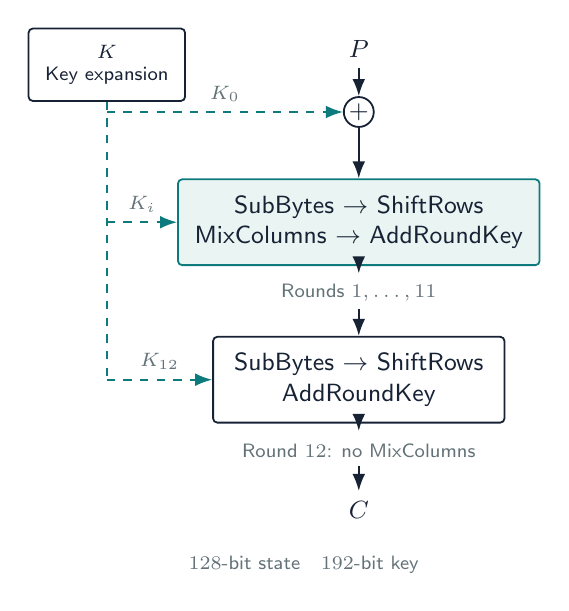
\begin{tikzpicture}
  \node (p) at (2.2,1.2) {$P$};
  \node[xor] (initial) at (2.2,.4) {$+$};
  \node[accent,minimum width=3.7cm] (rounds) at (2.2,-1) {SubBytes $\to$ ShiftRows\\MixColumns $\to$ AddRoundKey};
  \node[note] at (2.2,-1.9) {Rounds $1,\ldots,\AtlasPriorRounds$};
  \node[box,minimum width=3.7cm] (final) at (2.2,-3) {SubBytes $\to$ ShiftRows\\AddRoundKey};
  \node[note] at (2.2,-3.9) {Round $\AtlasRounds$: no MixColumns};
  \node (c) at (2.2,-4.65) {$C$};
  \draw[wire] (p) -- (initial); \draw[wire] (initial) -- (rounds);
  \draw[wire] (rounds.south) -- (2.2,-1.65);
  \draw[wire] (2.2,-2.1) -- (final); \draw[wire] (final.south) -- (2.2,-3.65);
  \draw[wire] (2.2,-4.1) -- (c);
  \node[box,minimum width=1cm,font=\sffamily\scriptsize] (schedule) at (-1,1) {$K$\\Key expansion};
  \draw[draw=atlasTeal,dashed] (schedule.south) -- (-1,-3);
  \draw[keywire] (-1,.4) -- node[above,note] {$K_0$} (initial);
  \draw[keywire] (-1,-1) -- node[above,note] {$K_i$} (rounds);
  \draw[keywire] (-1,-3) -- node[above,note] {$K_{\AtlasRounds}$} (final);
  \node[note] at (1.5,-5.35) {$128$-bit state\quad $\AtlasKeyBits$-bit key};
\end{tikzpicture}

\end{document}
